%%%%%%%%%%%%%%%%%%%%%%%%%%%%%%%%%%%%%%%%%%%%%%%%%%%%%%%%%%%%%%%%%%%
%
% First comes an example EPS file -- just ignore it and
% proceed on the \documentclass line
% your LaTeX will extract the file if required
%
\RequirePackage{fix-cm}
%
%\documentclass{svjour3}                     % onecolumn (standard format)
%\documentclass[smallcondensed]{svjour3}     % onecolumn (ditto)
\documentclass[smallextended]{svjour3}       % onecolumn (second format)
%\documentclass[twocolumn]{svjour3}          % twocolumn
%
\smartqed  % flush right qed marks, e.g. at end of proof
%
\usepackage{graphicx}
%
% \usepackage{mathptmx}      % use Times fonts if available on your TeX system
%
% insert here the call for the packages your document requires
%\usepackage{latexsym}
\usepackage{amsmath}
\usepackage{amssymb}
\usepackage{scalefnt}
\usepackage{graphicx}
\usepackage{hyperref}
\usepackage{subfigure}
\usepackage{enumerate}
\usepackage{caption}
\usepackage{booktabs}
\usepackage{natbib} 
\usepackage{lipsum}  
\usepackage{xfrac}
\usepackage{indentfirst}
\usepackage[brazil]{babel}
\hyphenation{re-gis-tra-dos}


\usepackage{color}
\usepackage[normalem]{ulem}
\definecolor{darkgreen}{RGB}{0,80,0}
\newcommand{\old}[1]{{\color{red}\sout{#1}}}
\newcommand{\new}[1]{{\color{blue}#1}}
\newcommand{\comment}[1]{{\color{darkgreen}{\bfseries [#1]}}}

% etc.
%
% please place your own definitions here and don't use \def but
% \newcommand{}{}
%
% Insert the name of "your journal" with
% \journalname{myjournal}
%
\begin{document}

\title{Tecnica $\sfrac{H}{V}$ para determinação da elipticidade da onda Rayleigh}
\subtitle{}

%\titlerunning{Dielectric permittivity effects in the detection of tree roots using GPR}        % if too long for running head

\author{Danilo Portela de Oliveira¹\and Marcelo Peres Rocha¹         
}

%\authorrunning{Short form of author list} % if too long for running head

\institute{Danilo Portela de Oliveira \at
              Campus Universitário Darcy Ribeiro - Universidade de Brasília - UnB, Asa Norte. %Prédio SG 13. \\
              %Tel.: +55 61 99287-5004\\
              %Fax: +123-45-678910
              \\
              \email{daniloportela97@gmail.com}           %  \\
%             \emph{Present address:} of F. Author  %  if needed
           %\and
           %Luísa Lins \at
             % Campus Universitário Darcy Ribeiro - Universidade de Brasília - UnB, Asa Norte. Prédio SG 13.
}

\date{¹Universidade de Brasília, UnB, Brasil}
% The correct dates will be entered by the editor


\maketitle

% -----------------------------------------------

\begin{abstract}

\lipsum[1]
\keywords{%Sismologia \and Ondas Rayleigh \and Arranjos sísmicos 
}
% \PACS{PACS code1 \and PACS code2 \and more}
% \subclass{MSC code1 \and MSC code2 \and more}
\end{abstract}

% -----------------------------------------------

\newpage

\section{Introdução}

A relação de ruído espectral horizontal para vertical (relação H/V) \citep{nakamura1989method} tem sido frequentemente usada para estudar a amplificação do local e a estrutura da crosta rasa e tem sido particularmente útil na avaliação de risco sísmico (por exemplo, \citealp{field1993theoretical}; \citealp{bonilla1997site}; \citealp{konno1998ground}; \citealp{riepl1998detailed}; \citealp{parolai2002new}; \citealp{bonnefoy2006nature}). No entanto, a relação H/V pode ser influenciada pela composição do campo de ondas de ruído (ou seja, Rayleigh, Love e ondas de corpo; consulte \citealp{bonnefoy2006nature} para uma revisão e \citealp{koper2010composition} para uma pesquisa global), dificultando a interpretação da relação H/V. A relação entre a elipticidade da onda Rayleigh (ou razão H/V da onda Rayleigh) com a estrutura rasa 1-D da Terra, por outro lado, está bem definida \citep{tanimoto2008zh}. 

A extração da elipticidade da onda de Rayleigh usando técnicas de matriz de 3 componentes tem se mostrado bastante confiável \citep{poggi2010estimating}. Recentemente, técnicas multicomponentes de correlação cruzada de ruído ambiental também foram desenvolvidas para obter medições robustas da relação de amplitude H/V da onda Rayleigh (\citealp{lin2014upper}; \citealp{lin20143}). Esta técnica mais recente usa correlações cruzadas de ruído entre pares de estações para aproximar as funções de Green da onda Rayleigh entre um par de estações onde uma estação é considerada uma fonte virtual e a outra estação é considerada um receptor. As correlações cruzadas podem então ser usadas para fazer observações da relação H/V da onda Rayleigh empregando uma força vertical ou radial na fonte virtual e medindo a relação de amplitude entre os componentes radial e vertical no receptor.

Embora a correlação cruzada de ruído tenha a vantagem de isolar as ondas de Rayleigh do ruído ambiental, a interpretação do resultado pode ser difícil se o campo de ruído não for semidifusivo. 
A aproximação de campo distante ajuda a garantir um campo de ruído semidifusivo, mas as estações de origem virtual devem estar a pelo menos três comprimentos de onda de distância das estações de destino. A incerteza da medição também pode ser alta se não houver estações suficientes atuando como fontes virtuais.

Então, este texto objetiva por meio de uma revisão bibliográfica (do artigo \citealp{ullah2016thickness}) exibir estudos utilizando este método em um local quase pantanoso, localizado em Colônia, na cidade de São Paulo, Brasil, para a estimativa da espessura do pacote de sedimentos não consolidados sobre o leito rochoso (embasamento neste caso). 

A técnica H/V é empregada no sítio em Colônia por causa de sua configuração geológica, pois possui um pacote espesso de sedimentos não consolidados sobrepostos a rochas duras do embasamento, essa interface não consolidada do solo rochoso dá origem a uma velocidade muito alta e contraste de densidade que é muito favorável para aplicação \textit{horizontal-over-vertical} (H/V).

% -----------------------------------------------

\section{Geologia do local}

A estrutura da Colônia está localizada na periferia sul da cidade de São Paulo, Brasil (Fig \ref{geologia}). Tem uma geometria circular (diâmetro de 3,6 km) compreendendo um anel anular de colinas que circundam uma depressão. A estrutura é majoritariamente um pântano. Sua origem é atribuída a um impacto de meteorito \citep{riccomini1989colonia}. A estrutura é formada em rochas do embasamento cristalino de idade neoproterozóica e a depressão é preenchida principalmente por sedimentos ricos em matéria orgânica de idade quaternária. Os principais tipos rochosos do embasamento compreendem xisto, quartzito, gnaisse, migmatito, diorito, quartzo-diorito \citep{sadowski1974tectonica}.

A profundidade total, estimada por investigação de reflexão sísmica (Fig \ref{geologia}), que não atingiu a parte central da estrutura \citep{riccomini2011colonia} é de cerca de 340 m (preenchimento sedimentar mais brecha). A função de velocidade de empilhamento nesta investigação (Fig \ref{fun_vel}) mostrou um incremento contínuo da velocidade da onda P com a profundidade, começando de aproximadamente 1500 m/s para 2150 m/s, o que é consistente com o aumento esperado da compactação dos sedimentos.

\begin{figure}[!hbtp]
  \begin{center}
  
  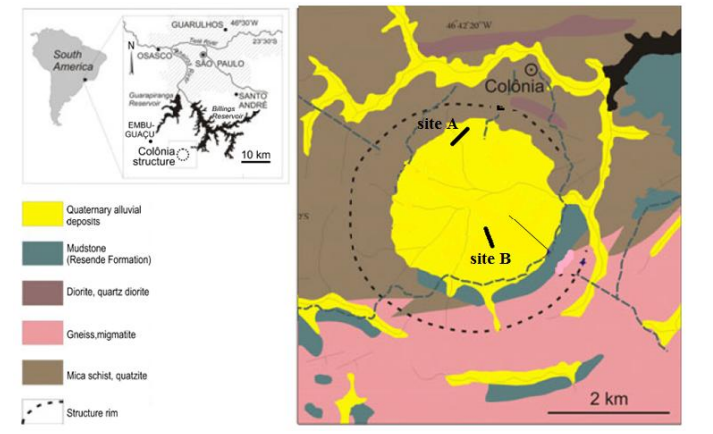
\includegraphics[scale=0.8]{Figures/fig1.png}
  \end{center}
  \caption{Localização (esquerda) e mapa geológico da estrutura da Colônia. As linhas grossas pretas indicam os locais dos testes MASW, enquanto as linhas finas indicam a linha de reflexão. (Modificado de \citealp{riccomini2011colonia}).
  }
  \label{geologia}
\end{figure}

\begin{figure}[!hbtp]
  \begin{center}
  
  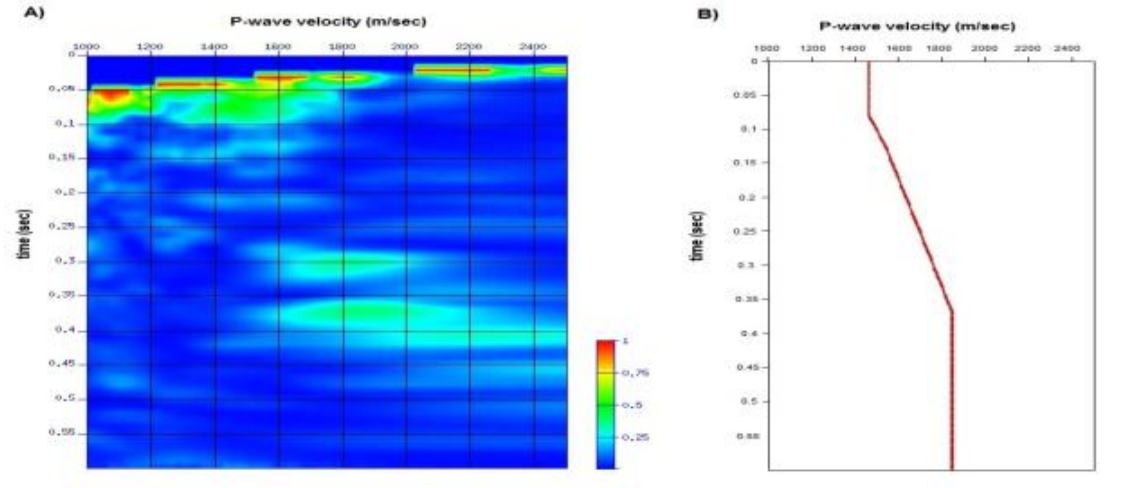
\includegraphics[scale=0.5]{Figures/fig2.png}
  \end{center}
  \caption{Figura com painel (A) e (B), onde a função de velocidade de empilhamento cdp é adquirido a 750 ms da investigação de reflexão sísmica de Colonia (onda P) (modificado de \citealp{riccomini2011colonia}).
  }
  \label{fun_vel}
\end{figure}

% -----------------------------------------------

\section{Metodologia}
\label{methods}

\subsection{Ondas Rayleigh}

As ondas Rayleigh são ondas de superfície que movimentam as partículas do meio de maneira polarizada ao longo de uma elipse vertical em sentido oposto ao da propagação (retrogrado). A razão entre as dimensões dos eixos horizontal e vertical da elipse de movimento de partícula define a elipticidade da onda Rayleigh, que é, sobre certas circunstâncias, dependente da estrutura local abaixo das estações \citep{berbellini2019constraining}.

\begin{figure}[!hbtp]
\begin{center}

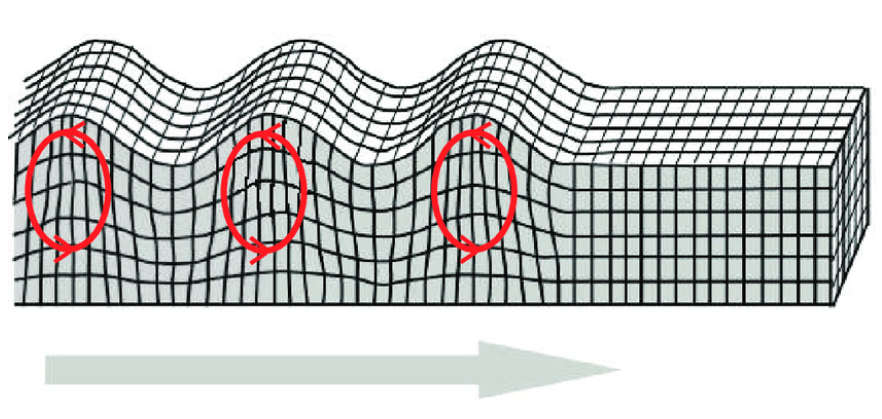
\includegraphics[scale=0.5]{Figures/ondas_rayleigh.png}
\end{center}
\caption{Comportamento das ondas Rayleigh na superfície terrestre \citep{de2009filtragem}.}
\label{ondas_rayleigh}
\end{figure}

\subsection{Elipticidade das Ondas Rayleigh}

Essa técnica, também chamada de Razão H/V da onda Rayleigh \citep{workman2017determination}, pode ser utilizada tanto para uma única estação, quanto para um arranjo de estações. A desvantagem conceitual da aplicação desse método para uma única estação é que, apesar de ser possível obter a elipse de movimento das partículas, não conseguem resolver a ambiguidade de 180 graus relacionada com a determinação do azimute reverso (backazimuth), não sendo possível identificar se o movimento é retrogrado ou não, e consequentemente, a direção de chegada das ondas Rayleigh (\citealp{workman2017determination}, \citealp{berbellini2019constraining}).

\subsection{inversão}

A partir de medidas do espectro H/V para diferentes períodos, é construída a curva de elipticidade média para as estações pertencentes ao arranjo. A curva de elipticidade é invertida para obtenção do modelo 1D de velocidade da onda S em relação à profundidade, logo abaixo do arranjo das estações (no centro do arranjo). Esse modelo pode ser interpretado em termos das descontinuidades existentes sob o arranjo das estações.

Para a inversão da elipticidade e para amostrar o espaço de parâmetros, utiliza-se o \textit{eighborhood algorithm} (NA) \citep{wathelet2008array} que é um método livre de derivadas em comparação com o método linearizado \citep{menke1989geophysical}. Este método (NA) auto-adaptativo amostra o espaço do modelo para encontrar um conjunto de modelos que melhor se ajusta aos dados reais. Para cada modelo amostrado, o algoritmo de inversão compara dados previstos com dados reais (usando a abordagem de modo normal de \cite{herrmann2013computer} para calcular curvas de elipticidade e avaliar uma função de custo). 

Dessa forma, o cálculo da função de custo leva em consideração o desajuste entre os dados reais e os valores previstos e geralmente também contém um termo para regularizar as soluções. Um termo de regularização é necessário quando a parametrização é feita de muitas camadas finas para promover os modelos mais suaves. A função custo é definida como:

\begin{equation}\label{eq:cost_function}
  c = \sum_{i=1}^{N_m} \frac{[d_{obs}^i - g^i(m)]^2}{(\sigma^i_{D})^2} + A \cdot N_m \sum_{j=1}^{N_L} [v_s^{j - 1} - 2v_s^{j} + v_s^{j + 1}]^2 
\end{equation}

Onde $d_{obs}^i$ são os dados observados, $g^i(m)$ são valores teóricos de elipticidade calculados usando um formalismo de modo normal para o modelo amostrado $m$, $\sigma^i_{D}$ é a variância da medição, $N_m$ é o número de medições, $N_L$ é o número de camadas, $A$ é um fator de escala e $v_s$ é a velocidade da onda de cisalhamento. 

O primeiro termo é o desajuste entre os dados observados e previstos, o segundo é o termo de regularização. $A$ é um fator de escala determinado por tentativa e erro: se $A$ for muito pequeno, os dados observados serão superajustados, enquanto o modelo resultante mostrará descontinuidades muito irrealistas. Por outro lado, se $A$ for muito grande, o modelo será plano e os dados observados não serão bem ajustados. Um bom fator $A$ produz modelos realistas enquanto ajusta bem os dados observados. 

%\subsection{Sample Collection}

%\subsection{Measuring Permittivity}

%\subsection{GPR Data Acquisition}

%\begin{figure}[!hbtp]
%\begin{center}

%\includegraphics[scale=0.5]{Figures/Fig1.png}
%\end{center}
%\caption{Acquisition with the 2.6 GHz antenna (GPR SIR 3000, Geophysical Survey System Inc - GSSI).}
%\label{acquisition}
%\end{figure}

% -----------------------------------------------

%\subsection{Data Processing}

%\emph{Header Gain Removal}

%\clearpage


%\begin{table}[!hbtp]
%\caption{Dielectric characteristics of common materials. Modified from \cite{alHagrey2007}, \cite{torgovnikov1993dielectric} and \cite{asprion1998ground}.}
%\label{table_alHagrey}
%\begin{tabular}{@{}lccc@{}}
%\toprule
%Material         & $\epsilon_{r}$ & $\sigma$ (mS m$^{-1}$) & $v$ (m ns$^{-1}$) \\ \midrule
%Sandy-loamy soil & 4 - 30         & 0.1 - 1000             & 0.05 - 0.18       \\
%Wood cellulose   & 4.5 - 22       & 0.24                   & 0.064 - 0.141     \\
%Fresh Water      & 81             & 0.1 - 10               & 0.03              \\
%Air              & 1              & 0                      & 0.3               \\ \bottomrule
%\end{tabular}
%\end{table}

%\begin{table*}[!hbtp]
%\caption{Permittivity values used in forward models.}
%\label{valores_modelosintetico}
%\centering
%\begin{tabular}{@{}ccc@{}}
%\toprule
%Model & Root Permittivity & Volumetric Root Water Content (\%) \\ \midrule
%1    & 2                   & 5                                  \\
%2    & 4                   & 15                                 \\
%3    & 8                   & 22                                 \\
%4    & 10                  & 28                                 \\
%5    & 15                  & 34                                 \\
%6    & 20                  & 46                                 \\
%7    & 25                  & 52                                 \\
%8    & 30                  & 60                                 \\
%9    & 80                  &  *\footnotemark[1]                                  \\ \bottomrule
%\end{tabular}
%\end{table*}
%\footnotemark[1]{Value used as an extrapolation to visualize how the model would behave, since the maximum saturation value is 70\%, which generates $\epsilon_{r} = 40$ \citep{guo2013cforward, hirano2009}.}

% -----------------------------------------------

\section{Resultados}
\label{results}

A partir de medidas do espectro H/V (componentes horizontais pelas verticais), para diferentes
períodos, espera-se construir a curva de elipticidade média para as estações pertencentes ao arranjo. A curva
de elipticidade será invertida para obtenção do modelo 1D de velocidade da onda S em relação à profundidade, logo abaixo do arranjo das estações (no centro do arranjo). Esse modelo pode ser interpretado em termos das descontinuidades existentes sob o arranjo das estações.

%\subsection{Experimental Data}

% -----------------------------------------------

\section{Discussões}


%\subsection{Experimental Data}

% -----------------------------------------------

\section{Conclusões}
\label{conclusions}


%\begin{acknowledgements}
%We would like to thank Dr. Welitom Rodrigues Borges for the assistance with data processing and for providing the antenna used in this research.  
%\end{acknowledgements}

%\clearpage
\bibliographystyle{seg}  % style file is seg.bst
\bibliography{References}

\end{document}

% -----------------------------------------------
